\chapter{Case study} \label{case-study}

It is certainly evident by now that this thesis is rather a practical implementation and an integration problem, than a research project. As one of the main goals is to combine different kind of data sources, it seems to be convenient from several aspects to have some data to work with. It makes the development easier, because we can see immediately, if the components can handle the data or that in what way they change it. The possession of sample inputs can also help to demonstrate the results and provides the capability of some independent verification.

% https://www.kaggle.com/selfishgene/historical-hourly-weather-data
I used the Historical Hourly Weather data set from Kaggle.com that contains hourly measurement results of various weather attributes, such as temperature, humidity, air pressure, etc. The data is available from several cities from the USA, Canada and Israel from October 2012 to November 2017 \cite{kaggle-data}.

\begin{figure}[h]
	\centering
	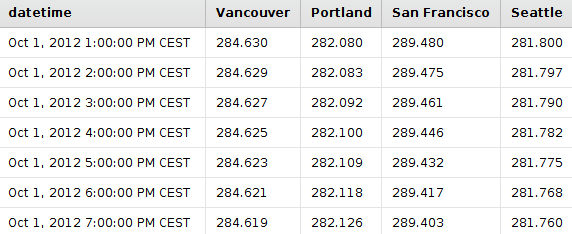
\includegraphics[width=130mm, keepaspectratio]{figures/weather-data-extract.png}
	\caption{Extract from the temperature data set}
	\label{fig:weather-data-extract}
\end{figure}

%---
\section{RapidMiner source}
%---

Concerning the part of the RapidMiner Server, it exposes a process that provides the temperature data from the sample data set. It accepts a parameter determining from which city the user wants to acquire this information. In short, it provides a filtering option by city.

%---
\section{Python source} \label{case-study-python-source}
%---

In this project I demonstrate a proof-of-concept use-case, when the Python data source component reads information from a database and also from an external API service. To be more precise, in the database I store the measured daily minimum and maximum temperature data from 2012 to 2017 in New York. Concerning the the API part, I created a small web application with a REST API that exposes historical highest and lowest temperature values for a given day of the year, also in New York. In the middleware written in Python, I implemented an example business logic which counts on how many days in a month (from October 2012 to November 2017) the measured temperature got close to the all-time records. I have to mention, that the calculation of these historical highest and lowest values is also heuristic. I only took data from January 1959 to September 2012 into account.

I believe, that this is a quite common problem, to have some data in one's storage, but for a better business competence, the usage of external services is also necessary. Hence, this example set-up could serve as an applicable demonstration for further possibilities.